\vspace{-1EX}
\begin{figure}[tb]
\centering
\begin{subfigure}[t]{0.47\textwidth}
    \centering
    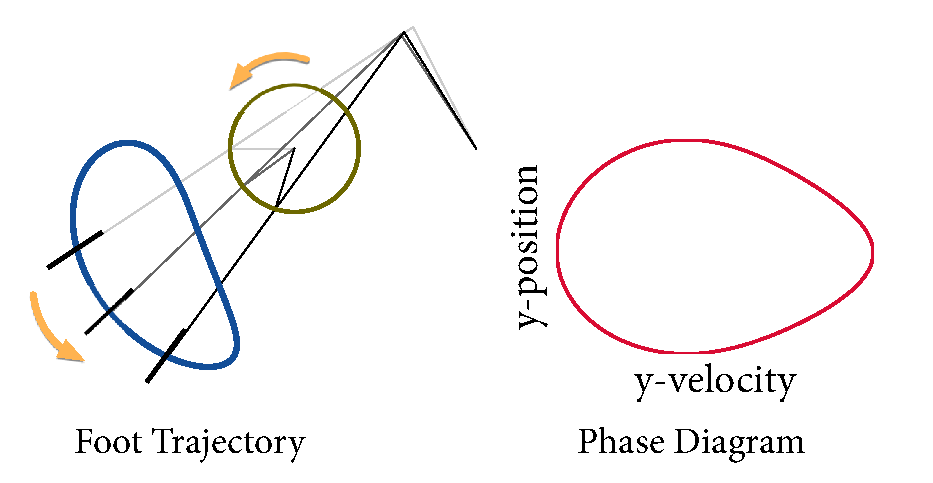
\includegraphics[width = \textwidth]{foot_traj_orig.eps}
    \caption{Robot foot locus and phase portrait}
    \label{fig:trajrob}
\end{subfigure}
\quad
\begin{subfigure}[t]{0.47\textwidth}
    \centering
    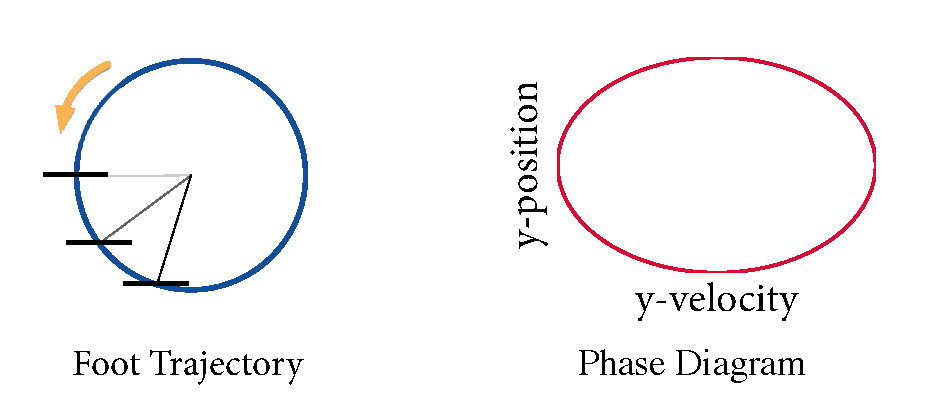
\includegraphics[width = \textwidth]{foot_traj_simple.eps}
    \caption{Simplified foot locus and phase portrait} 
    \label{fig:trajsimp}
\end{subfigure}
\vspace{0.5EX}
\caption{Real and simplified leg trajectories (blue) and phase portraits (red).}
\label{fig:traj}
\end{figure}

\textcolor{prime}{\textsf{Leg Model}}
\begin{itemize}
    \item Only considers time-averaged vertical forces generated in one cycle of a simplified trajectory
    \item Assumes velocity of legs $\gg$ velocity of body oscillations
    \item Allows for different foot velocties during the downwards and upwards phases of the trajectory
    \item We integrate the following force equation~\cite{glasheen1996vertical} over the simplified trajectory
        \begin{equation}
            F(t) = - C_D^* \left[\frac{1}{2} S \rho \dot{y}_f(t) |\dot{y}_f(t) | + S \rho g y_f(t) \right]
            \label{eq:force_t}
        \end{equation}
\hspace{1EM} $C_D^*$ drag coefficient, $S$ area of foot, $\rho$ water density, $y_f$ position of foot, \\ \hspace{1EM} $g$ acceleration of gravity
\end{itemize}
\vspace{1EX}

\textcolor{prime}{\textsf{Robot Model}} \\
We linearize the result of integrating equation~\ref{eq:force_t} and write the height and roll dynamics of the robot in the form

\begin{equation}
    M \ddot{\vec{y}} = A \vec{y} + G + B \vec{\omega} 
    \label{eq:rob_dyn}
\end{equation}

\hspace{1EM} $\vec{y} = [y, \theta]^T = $\  height and roll \\

\hspace{1EM} $\vec{\omega} = [\omega^-_l, \omega^+_l, \omega^-_r, \omega^+_r]^T = $\ plunge and retract leg frequencies for left \\ \hspace{1EM} and right sides of robot
